% Training Window Ablation Results
% Replaces: tab:training-window-ablation-results in appendix_c
% Grouped bar chart comparing 4 training window scenarios

\begin{figure}[htbp]
\centering
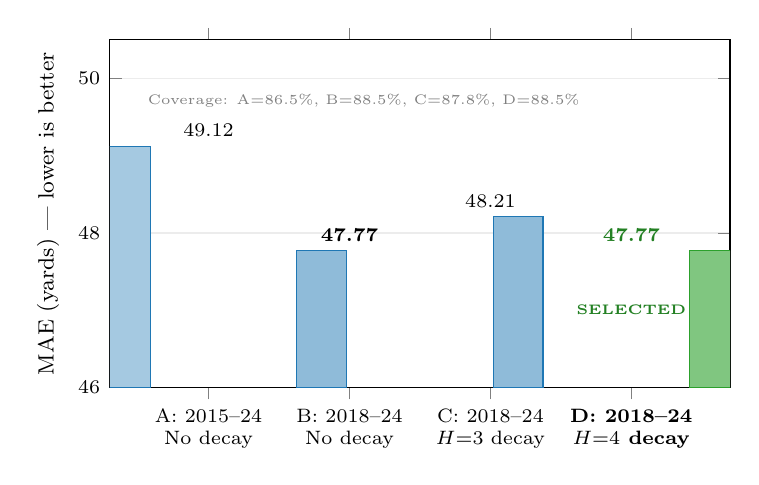
\begin{tikzpicture}
\definecolor{accent}{RGB}{31,119,180}
\definecolor{accentGreen}{RGB}{44,160,44}

\begin{axis}[
  width=0.78\textwidth,
  height=6cm,
  ybar,
  bar width=18pt,
  ylabel={MAE (yards) --- lower is better},
  ylabel style={font=\footnotesize},
  ymin=46, ymax=50.5,
  xtick={1,2,3,4},
  xticklabels={
    {\shortstack{A: 2015--24\\No decay}},
    {\shortstack{B: 2018--24\\No decay}},
    {\shortstack{C: 2018--24\\$H{=}3$ decay}},
    {\shortstack{\textbf{D: 2018--24}\\\textbf{$H{=}4$ decay}}}
  },
  xticklabel style={font=\scriptsize},
  yticklabel style={font=\scriptsize},
  grid=major,
  grid style={gray!15},
  xmajorgrids=false,
  enlarge x limits={abs=0.7},
]

% MAE bars
\addplot[fill=accent!40, draw=accent] coordinates {(1, 49.12)};
\addplot[fill=accent!50, draw=accent] coordinates {(2, 47.77)};
\addplot[fill=accent!50, draw=accent] coordinates {(3, 48.21)};
\addplot[fill=accentGreen!60, draw=accentGreen] coordinates {(4, 47.77)};

% Value labels
\node[font=\scriptsize, anchor=south] at (axis cs:1,49.12) {49.12};
\node[font=\scriptsize\bfseries, anchor=south] at (axis cs:2,47.77) {47.77};
\node[font=\scriptsize, anchor=south] at (axis cs:3,48.21) {48.21};
\node[font=\scriptsize\bfseries, text=accentGreen!80!black, anchor=south] at (axis cs:4,47.77) {47.77};

% Selected annotation
\node[font=\tiny\bfseries, text=accentGreen!80!black, anchor=north] at (axis cs:4,47.2)
  {SELECTED};

% Coverage annotation
\node[font=\tiny, text=black!50, anchor=south west, align=left] at (axis cs:0.5,49.5)
  {Coverage: A=86.5\%, B=88.5\%, C=87.8\%, D=88.5\%};

\end{axis}
\end{tikzpicture}
\caption[Training window ablation]{Training window ablation (2025 holdout, $n=148$ QB-games). Scenario D (2018--2024, $H=4$ exponential decay) ties Scenario B at 47.77 yards MAE but is preferred for incorporating historical context with gentle decay. Removing pre-2018 data (A$\to$B) reduces MAE by 1.35 yards; adding moderate decay further improves calibration coverage (88.5\%).}
\label{fig:training-window-chart}
\end{figure}
